\section{Колебательно-вращательные гамильтонианы в молекулярной системе координат}

При выводе молекулярного гамильтониана полиатомной системы часто предполагается, что амплитуда колебаний мала. Гамильтониан, полученный Вильсоном и Говардом, для системы с колебаниями малой амплитуды широко используется и часто служит базисом для дальнейших уточнений. \par
Однако колебания большой амплитуды, проявляющиеся в в слабосвязанных комплексах не могут быть описаны при помощи того же подхода. Для описания колебаний большой амплитуды часто используются координаты Якоби, координаты Радау, гиперсферические координаты и др. \par 
Рассмотрим систему из $N$ частиц с массами $\lb m_1, \dots m_N \rb$ и координатами $\lb \mf{r}_1, \dots, \mf{r}_N \rb$ в лабораторной системе координат. Лагранжева кинетическая энергия в лабораторной системе координат записывается как
\begin{gather}
    T_\text{tot} = \frac{1}{2} \sum_{k = 1}^N m_k \dot{\mf{r}}_k^2.
\end{gather}

Чтобы отделить трансляционные степени свободы введем координаты Якоби \cite{greiner, littlejohn1995}, являющиеся обобщением координат, используемых в двухатомных системах. Переход к трансляционно-инвариантному набору координат может быть осуществлен следующим образом \cite{greiner}
\begin{gather}  
    \lc
    \begin{aligned}
        \bs{\rho}_1 &= \frac{m_1 \mf{r}_1}{m_1} - \mf{r}_2 = \mf{r}_1 - \mf{r}_2, \\
        \bs{\rho}_2 &= \frac{m_1 \mf{r}_1 + m_2 \mf{r}_2}{m_1 + m_2}, \\
        \mf{\rho}_j &= \frac{\displaystyle \sum_{k = 1}^j m_k \mf{r}_k}{\displaystyle \sum_{k = 1}^j m_k} - \mf{r}_{j + 1}, \quad 2 < j < N \\
        \mf{\rho}_N &= \frac{1}{M} \sum_{k = 1}^N m_k \mf{r}_k,
    \end{aligned}
    \right.
\end{gather}
%
где через $M$ обозначена суммарная масса системы частицы. \par
Первый вектор Якоби $\bs{\rho}_1$ соединяет частицы 1 и 2. Второй вектор Якоби соединяет центр масс первых двух частиц и третью частицу. Третий вектор Якоби соеднияет центр масс первых трех частиц и четвертую частицу и т.д. Последний вектор Якоби суть вектор, направленный в центр масс системы. Пример векторов Якоби для системы, соcтоящей из трех частиц, приведен на Рис. \ref{fig:jacobi_coordinates}. 

\begin{figure}
    \centering
    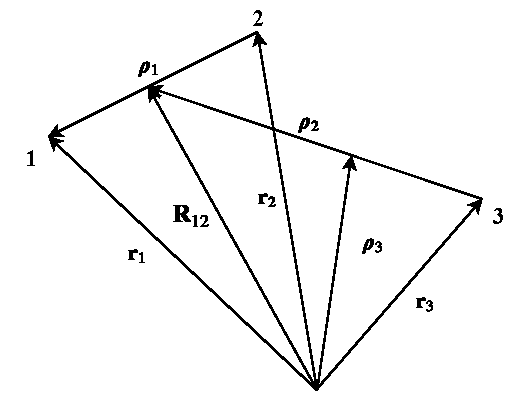
\includegraphics[width=0.5\linewidth]{pictures/jacobi_coordinates.pdf}
    \caption{Координаты Якоби  для системы из 3 частиц, пронумерованных 1, 2, 3. Через $\mf{R}_{12}$ бозначен вектор, направленный в центр масс пары частиц 1 и 2.}
    \label{fig:jacobi_coordinates}
\end{figure}

Можно показать, что кинетическая энергия в лагранжевой форме, выраженная через векторы Якоби записывается как \cite{greiner} 
\begin{gather}
    T_\text{tot} = \frac{1}{2} M \dot{\bs{\rho}}_N^2 + \frac{1}{2} \sum_{k = 1}^{N - 1} \mu_k \dot{\bs{\rho}}_k^2,
\end{gather}
%
где приведенные массы $\mu_j$ связаны с исходными массами $m_j$ следующими соотношениями
\begin{gather}
    \frac{1}{\mu_j} = \frac{1}{M_j} + \frac{1}{m_{j+1}}, \quad M_j = \sum_{k = 1}^j m_k, \quad j = 1 \dots N - 1. \label{polyatom-jacobi-masses}
\end{gather}

Данная последовательность введения векторов Якоби не является единственно возможной. Выбор векторов Якоби в каждом отдельном случае обусловлен структурой рассматриваемой системы. Описанная последовательность является общим случаем, в котором получена кинетическая энергия для системы из $N$ частиц. При другом выборе векторов Якоби общая форма кинетической энергии сохранится, однако изменятся приведенные массы $\mu_j$. \par
Отделяя центр масс, мы приходим к следующей форме кинетической энергии
\begin{gather}
    \Tl = \frac{1}{2} \sum_{k = 1}^{N - 1} \mu_k \dot{\bs{\rho}}_k^2.
\end{gather}

Для отделения вращательных степеней свободы введем подвижную систему координат. Лабораторная и подвижная системы координат связаны друг с другом матрицей ортогонального преобразования $\bbS$ \cite{goldstein}. Обозначим через $\mf{R}_j$ координаты векторов Якоби в подвижной системе координат. Введенные векторы $\mf{R}_j$ связаны с векторами в лабораторной системе линейным преобразованием
\begin{gather}
    \boldsymbol{\rho}_j = \bbS \mf{R}_j.
\end{gather}
Будем рассматривать параметризацию матрицы ортогонального преобразования $\bbS$ тройкой углов Эйлера $\Phi$, $\Theta$, $\Psi$ \cite{goldstein}
\begin{gather}
    \bbS = 
    \begin{bmatrix}
        \cos \Psi \cos \Phi - \cos \Theta \sin \Phi \sin \Psi & -\sin \Psi \cos \Phi - \cos \Theta \sin \Phi \cos \Psi & \sin \Theta \sin \Phi \\ 
        \cos \Psi \sin \Phi + \cos \Theta \cos \Phi \sin \Psi & -\sin \Psi \sin \Phi + \cos \Theta \cos \Phi \cos \Psi & - \sin \Theta \cos \Phi \\
        \sin \Theta \sin \Psi & \sin \Theta \cos \Psi & \cos \Theta
    \end{bmatrix}.
\end{gather}

Лагранжева кинетическая энергия в подвижной системе отсчета может быть записана как \cite{landau-volume1}
\begin{gather}
    \Tl = \frac{1}{2} \sum_{i = 1}^{N-1} \mu_i \dot{\mf{R}}_i^2 + \frac{1}{2} \sum_{i = 1}^{N - 1} \mu_i \lsq \boldsymbol{\Omega} \times \mf{R}_i \rsq^2 + \boldsymbol{\Omega}^{+} \sum_{i = 1}^{N - 1} \mu_i \lsq \mf{R}_i \times \dot{\mf{R}}_i \rsq,
\end{gather}
%
где $\boldsymbol{\Omega}$ -- вектор угловой скорости в проекции на подвижную систему координат. Вектор угловой скорости $\boldsymbol{\Omega}$ связан с углами Эйлера и эйлеровыми скоростями следующим соотношением
\begin{gather}
    \boldsymbol{\Omega} = \bbV \mf{v} = 
    \begin{bmatrix}
        \sin \Theta \sin \Psi & \cos \Psi & 0 \\
        \sin \Theta \cos \Psi & -\sin \Psi & 0 \\
        \cos \Theta & 0 & 1 
    \end{bmatrix}
    \begin{bmatrix}
        \dot{\Phi} \\ \dot{\Theta} \\ \dot{\Psi}
    \end{bmatrix}. \label{polyatom-matrixV}
\end{gather}

Введем набор внутренних координат $\mf{q} = \lb q_1, \dots q_s \rb$ и, используя связь координат Якоби с введенными координатами $\mf{R}_j = \mf{R}_j(\mf{q})$, перепишем выражение для кинетической энергии в форме \cite{petrov2015}
\begin{gather}
    \Tl = \frac{1}{2} \dot{\mf{q}}^+ \bba \dot{\mf{q}} + \bOmega^+ \bbA \mf{q} + \frac{1}{2} \bOmega^+ \bbI \, \bOmega, \label{body-fixed-lagrange-energy} 
\end{gather}
%
где через $\bba, \bbA, \bbI$ обозначены матрица относительной кинетической энергии, кориолисова матрица и матрица тензора инерции, соответственно. Элементы матриц относительной кинетической энергии и кориолисова взаимодействия заданы следующими выражениями
\begin{gather}
    \bba_{jk} = \sum_{i = 1}^{N - 1} \mu_i \frac{\partial \mf{R}_i}{\partial q_j} \frac{\partial \mf{R}_i}{\partial q_k}, \quad \bbA_{jk} = \sum_{i = 1}^{N - 1} \mu_i \lsq \mf{R}_i \times \frac{\partial \mf{R}_i}{\partial q_k} \rsq_j. \label{polyatom-kinetic-energy-matrices}
\end{gather}

Выражение для кинетической энергии \eqref{body-fixed-lagrange-energy} для перехода к Гамильтоновой форме удобно переписать в матричном виде
\begin{gather}
    \Tl = \frac{1}{2} \begin{bmatrix} \bOmega^+ & \dot{\mf{q}}^+ \end{bmatrix} \bbB \begin{bmatrix} \bOmega \\ \dot{\mf{q}} \end{bmatrix}, \label{polyatom-block-matrix-kin-energy}
\end{gather}
%
где через $\bbB$ обозначена блочная матрица со следующими элементами 
\begin{gather}
    \bbB = \begin{bmatrix} 
    \bbI & \bbA \\ \bbA^+ & \bba 
    \end{bmatrix}.
\end{gather}

Можно показать, что если ввести величину $\mf{J}$ как производную кинетической энергии в лагранжевой форме $\Tl$ по вектору угловой скорости $\bOmega$, то $\mf{J}$ суть вектор углового момента в подвижной системе координат (приложение \ref{appendix:angular-momentum-body-fixed}). Обобщенные импульсы $\mf{p}$, сопряженные координатам $\mf{q}$, по определению ранвы производным кинетической энергии в лагранжевой форме $\Tl$ по обобщенным скоростям $\dot{\mf{q}}$: 
\begin{gather}
    \mf{J} = \frac{\partial \Tl}{\partial \bOmega} = \bbI \bOmega + \bbA \dot{\mf{q}}, \label{polyatom-angmom1} \\
\mf{p} = \frac{\partial \Tl}{\partial \dot{\mf{q}}} = \bbA^+ \bOmega + \bba \dot{\mf{q}} \label{polyatom-gen-momenta}.
\end{gather}

Заметим, что выражения \eqref{polyatom-angmom1}, \eqref{polyatom-gen-momenta} могли быть получены дифференцированием выражения  \eqref{polyatom-block-matrix-kin-energy} по блочному вектору с компонентами $\bOmega$ и $\dot{\mf{q}}$. Выражения для углового момента и обобщенных импульсов объединим в один блочный вектор
\begin{gather}
    \begin{bmatrix} \mf{J} \\ \mf{p} \end{bmatrix} = \bbB \begin{bmatrix} \bOmega \\ \dot{\mf{q}} \end{bmatrix} = 
    \begin{bmatrix} \bbI & \bbA \\ \bbA^+ & \bba \end{bmatrix} \begin{bmatrix} \bOmega \\ \dot{\mf{q}} \end{bmatrix}.
\end{gather}

Для того, чтобы выразить лагранжевы переменные из полученного выражения, нам необходимо обратить блочную матрицу $\bbB$. Это обращение удобно выполнить при помощи формул Фробениуса \cite{petrov2015, gantmaher}. Через $\bbG$ обозначают обратную матрицу к $\bbB$, ее матричные компоненты выражаются как
\begin{gather}
    \begin{aligned}
        \bbG_{11} &= \lb \bbI - \bbA \bba^{-1} \bbA^+ \rb^{-1} \\
        \bbG_{12} &= -\bbI^{-1} \bbA \bbG_{22} = -\bbG_{11} \bbA \bba^{-1} \\
        \bbG_{21} &= -\bba^{-1} \bbA^+ \bbG_{11} = \bbG_{22} \bbA^+ \bbI^{-1} \\
        \bbG_{22} &= \lb \bba - \bbA^+ \bbI^{-1} \bbA \rb^{-1}
    \end{aligned} \label{polyatom-frobenius}
\end{gather}

Переход от кинетической энергии в форме Лагранжа к кинетической энергии в форме Гамильтона осуществляем при помощи стандартной процедуры \cite{goldstein}
\begin{gather}
    \Th = \begin{bmatrix} \bOmega^+ & \dot{\mf{q}}^+ \end{bmatrix} \begin{bmatrix} \mf{J} \\ \mf{p} \end{bmatrix} - \Tl = \frac{1}{2} \begin{bmatrix} \mf{J}^+ & \mf{p}^+ \end{bmatrix} \bbG \begin{bmatrix} \mf{J} \\ \mf{p} \end{bmatrix} = \frac{1}{2} \mf{J}^+ \bbG_{11} \mf{J} + \mf{J}^+ \bbG_{12} \mf{p} + \frac{1}{2} \mf{p}^+ \bbG_{22} \mf{p}, \label{general-rovibrational-kin-energy} 
\end{gather}
а полный колебательно-вращательный гамильтониан получается в результате добавления потенциальной энергии
\begin{gather}
    H = \frac{1}{2} \mf{J}^+ \bbG_{11} \mf{J} + \mf{J}^+ \bbG_{12} \mf{p} + \frac{1}{2} \mf{p}^+ \bbG_{22} \mf{p} + U(\mf{q}). \label{general-rovibrational-hamiltonian} 
\end{gather}

В данной работе мы будем рассматривать системы, состоящие из жесткой линейной молекулы атома и из двух жестких линейных молекул. \par
В случае системы линейная молекула$-$атом построим вектор Якоби вдоль линейной молекулы, тогда второй вектор Якоби соединяет центр масс линейной молекулы с атомом. Определим подвижную систему координат таким образом, чтобы построенные вектора Якоби $\mf{R}_1$, $\mf{R}_2$ задавали плоскость $OXZ$ подвижной системы. Дополнительно потребуем, чтобы вектор $\mf{R}_2$, соединяющий центр масс линейной молекулы с атомом, лежал вдоль оси $OZ$ (см. рис. \ref{fig:body-fixed-linear-atom}). Такое определение системы координат известно как $R$-вложение \cite{tennyson1986}. Обозначим длину линейной молекулы через $l$.
    
\begin{figure}[H]
    \centering
    %\begin{minipage}{0.49\linewidth}
    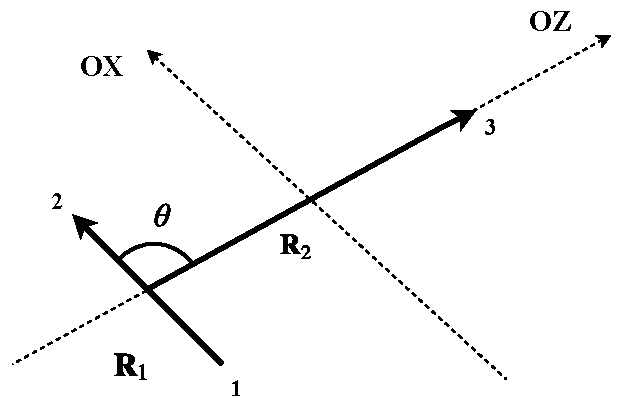
\includegraphics[width=0.5\linewidth]{pictures/triatom_coordinates.pdf}
    %\end{minipage}
    %\begin{minipage}{0.49\linewidth}
    %    Взять картинку из будущей статьи с N$_2$-N$_2$
    %\end{minipage}
    \caption{Молекулярная система координат для системы линейная молекула-атом}
    \label{fig:body-fixed-linear-atom}
\end{figure}

В качестве обобщенных координат выберем $R$ -- длину вектора Якоби $\mf{R}_2$ или, что эквивалентно, расстояние от атома до центра масс линейной молекулы, и угол $\theta$ между векторами Якоби $\mf{R}_1$ и $\mf{R}_2$. Выпишем координаты векторов в подвижной системе через обобщенные координаты $\mf{q} = \lb R, \theta \rb$: 
\begin{gather}
    \begin{aligned}
        X_1 &= l \sin \theta \\
        Y_1 &= 0 \\
        Z_1 &= l \cos \theta
    \end{aligned} \qquad
    \begin{aligned}
        X_2 &= 0 \\ 
        Y_2 &= 0 \\
        Z_2 &= R 
    \end{aligned}. \label{linear-molecule-atom-jacobi-coords}
\end{gather}

Вывод дальнейших выражений реализовывался в системе компьютерной алгебры Maple. Координаты векторов Якоби \eqref{linear-molecule-atom-jacobi-coords} использовались для расчета компонент матриц относительной кинетической энергии, кориолисова взаимодействия и тензора инерции по выражениям \eqref{polyatom-kinetic-energy-matrices}. В случае линейная молекула$-$атом блоки матрицы $\bbG$ могут быть получены в компактном виде. Уже для случая двух жестких линейных молекул выражения для блоков матрицы $\bbG$ оказываются слишком громоздкими, поэтому была разработана схема реализации траекторного расчета, избегающая аналитической работы с компонентами этих матриц, переносимая на системы с произвольным количеством вращательных степеней свободы. \par
В качестве примера системы линейная молекула$-$атом мы выбрали CO$_2-$Ar. Внутримолекулярные колебания молекулы CO$_2$ происходят существенно быстрее межмолекулярных движений комплекса с атомом аргона, поэтому предполагается, что взаимодействие между внутри- и межмолекулярными колебательными модами в данном случае компенсируется. \par
Приведенные массы частиц Якоби согласно \eqref{polyatom-jacobi-masses} равны
\begin{gather}
    \mu_1 = \frac{m_1}{2}, \quad \mu_2 = \frac{m_2 \lb 2 m_1 + m_3 \rb}{2 m_1 + m_2 + m_3},
\end{gather}
% 
где через $m_1$ обозначена масса атома кислорода, через $m_2$ -- масса атома аргона, через $m_3$ -- масса атома углерода. \par
При помощи системы компьютерной алгебры были получены следующие выражения для матриц кинетической энергии в форме Лагранжа
\begin{gather}
	\bba =
	\begin{bmatrix}
		\mu_2 & 0 \\
		0 & \mu_1 l^2
	\end{bmatrix}, \quad 
	\bbA = 
	\begin{bmatrix}
		0 & 0 \\
		0 & \mu_1 l^2 \\
		0 & 0 
	\end{bmatrix}, \quad
	\bbI = 
	\begin{bmatrix}
		\mu_1 l^2 \cos^2 \theta + \mu_2 R^2 & 0 & -\mu_1 l^2 \sin \theta \cos \theta \\
		0 & \mu_1 l^2 + \mu_2 R^2 & 0 \\
		- \mu_1 l^2 \sin \theta \cos \theta & 0 & \mu_1 l^2 \sin^2 \theta
	\end{bmatrix}. \notag
\end{gather}

Подставив полученные выражения для матриц в формулы Фробениуса \eqref{polyatom-frobenius}, приходим к следующим выражениям для матриц, определяющим кинетическую энергию в форме Гамильтона 
\begin{gather}
	\bbG_{11} =
	\begin{bmatrix}
		\dfrac{1}{\mu_2 R^2} & 0 & \dfrac{\ctg \theta}{\mu_2 R^2} \\
		0 & \dfrac{1}{\mu_2 R^2} & 0 \\
		\dfrac{\ctg \theta}{\mu_2 R^2} & 0 & \dfrac{\ctg^2 \theta}{\mu_2 R^2} + \dfrac{1}{\mu_1 l^2 \sin^2 \theta}
	\end{bmatrix}, \quad
	\bbG_{12} =
	\begin{bmatrix}
		0 & 0 \\
		0 & - \dfrac{1}{\mu_2 R^2} \\
		0 & 0
	\end{bmatrix}, \quad 
	\bbG_{22} = 
	\begin{bmatrix}
		\dfrac{1}{\mu_2} & 0 \\
		0 & \dfrac{1}{\mu_2 R^2} + \dfrac{1}{\mu_1 l^2}
	\end{bmatrix}. \notag
\end{gather}

Итак, кинетическая энергия в форме Гамильтона для системы CO$_2-$Ar в выбранной нами молекулярной системе отсчета получается следующей
\begin{gather}
\Th = \frac{1}{2 \mu_2} p_R^2 + \lb \frac{1}{2 \mu_2 R^2} + \frac{1}{2 \mu_1 l^2} \rb p_\theta^2 - \frac{1}{\mu_2 R^2} p_\theta \Jy + \frac{1}{2 \mu_2 R^2} \Jy^2 + \frac{1}{2 \mu_2 R^2} \Jx^2 + \frac{1}{2 \sin^2 \theta} \lb \frac{\cos^2 \theta}{\mu_2 R^2} + \frac{1}{\mu_1 l^2} \rb \Jz^2 + \notag \\
+ \frac{\ctg \theta}{\mu_2 R^2} \Jx \Jz. 
\end{gather}

В случае системы, состоящей из двух жестких линейных молекул, удобно построить векторы Якоби вдоль каждой из линейных молекул, тогда третий вектор соединяет их центры масс. Определим подвижную систему координат таким образом, чтобы вектор, соединяющий центры масс линейных молекул, лежал на оси $OZ$ подвижной системы. Потребуем, чтобы вектор, определяющий одну из линейных молекул, лежал в плоскости $OXZ$ подвижной системы (Рис. \ref{fig:two-linear-molecules-body-fixed}). Вторая молекула при этом может выходить из плоскости подвижной системы -- для того, чтобы описать ее ориентацию необходимо ввести два угла, тогда как для описания ориентации первой молекулы достаточно одного полярного угла. Введя таким образом систему координат мы заведомо сделали линейные молекулы неравноправными, так что соответствующие им координаты будут входить в кинетическую энергию неодинаковым образом. Обозначим длины линейных молекул через $l_1$ и $l_2$, соответственно. В качестве обобщенных координат выберем $R$ -- расстояние между центрами масс линейных молекул, $\theta_1$, $\theta_2$ -- полярные углы линейных молекул в плоскости $OXZ$, $\varphi$ -- угол между плоскостью $OXZ$ и плоскостью, заданной молекулой, выходящей из плоскости подвижной системы, и центром масс второй молекулы.

\begin{figure}[H]
    \centering
    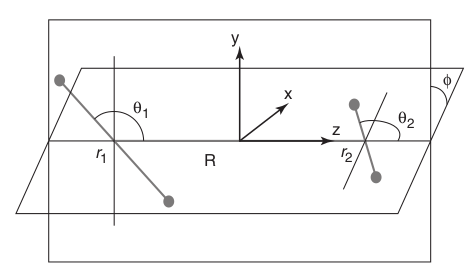
\includegraphics[width=0.5\linewidth]{pictures/n2n2_coordinate_frame.png}
    \caption{Молекулярная система координат для системы из двух линейных молекул; взять картинку из драфта статьи?}
    \label{fig:two-linear-molecules-body-fixed}
\end{figure}

Выпишем координаты векторы Якоби в подвижной системе через обобщенные координаты $\mf{q} = \lb R, \theta_1, \varphi, \theta_2 \rb$:
\begin{gather}
    \begin{aligned}
        X_1 &= l_1 \sin \theta_1 \\
        Y_1 &= 0 \\
        Z_1 &= l_1 \cos \theta_1 
    \end{aligned} \qquad
    \begin{aligned}
        X_2 &= l_2 \cos \varphi \sin \theta_2 \\
        Y_2 &= l_2 \sin \varphi \sin \theta_2 \\
        Z_2 &= l_2 \cos \theta_2
    \end{aligned} \qquad
    \begin{aligned}
        X_3 &= 0 \\
        Y_3 &= 0 \\
        Z_3 &= R
    \end{aligned} \label{polyatom-linear-linear-coordinates}
\end{gather}

В качестве примера системы, состоящей из двух линейных молекул, выбрана N$_2-$N$_2$. Приведенные масс частиц Якоби равны
\begin{gather}
    \mu_1 = \frac{m}{2}, \quad \mu_2 = \frac{m}{2}, \quad \mu_3 = 2m, \label{polyatom-n2n2-jacobi-masses}
\end{gather}
%
где через $m$ обозначена масса атома азота. Длины линейных молекул в дальнейшем обозначаются одинаково $l = l_1 = l_2$.

Выражения для матриц кинетической энергии в форме Лагранжа были получены из \eqref{polyatom-linear-linear-coordinates} при помощи системы компьютерной алгебры. Введенный набор координат является ортогональным, т.к. матрица относительной кинетической энергии оказывается диагональной. Приводим выражения для случая двух произвольных линейных молекул через массы частиц Якоби; выражения для конкретного случая N$_2-$N$_2$ получаются в результате подстановки масc \eqref{polyatom-n2n2-jacobi-masses}.  
\begin{gather}
\bba = 
\begin{bmatrix}
\mu_3 & 0 & 0 & 0 \\
0 & \mu_2 l_2^2 \sin \theta_2 & 0 & 0 \\
0 & 0 & \mu_1 l_1^2 & 0 \\
0 & 0 & 0 & \mu_2 l_2^2 \\ 
\end{bmatrix}, \quad  
\bbA = 
\begin{bmatrix}
0 & -\mu_2 l_2^2 \cos \varphi \sin \theta_2 \cos \theta_2 & 0 & -\mu_2 l_2^2 \sin \varphi  \\
0 & -\mu_2 l_2^2 \sin \varphi \sin \theta_2 \cos \theta_2 & \mu_1 l_1^2 & \mu_2 l_2^2 \cos \varphi \\
0 &  \mu_2 l_2^2 \sin^2 \theta_2 & 0 & 0
\end{bmatrix} \notag 
\end{gather}

Компоненты матрицы тензора инерции в подвижной системе отсчета получаются следующие
\begin{gather}
    \begin{aligned}
        I_{XX} &= \mu_1 l_1^2 \cos^2 \theta_1 + \mu_2 l_2^2 (\sin^2 \varphi \sin^2 \theta_2 + \cos^2 \theta_2) + \mu_3 R^2, \\ 
        I_{XY} &= -\mu_2 l_2^2 \sin \varphi \cos \varphi \sin^2 \theta_2, \\ 
        I_{XZ} &= -\mu_1 l_1^2 \sin \theta_1 \cos \theta_1 - \mu_2 l_2^2 \cos \varphi \sin \theta_2 \cos \theta_2, \\
        I_{YY} &= \mu_1 l_1^2 + \mu_2 l_2^2 (\cos^2 \varphi \sin^2 \theta_2 + \cos^2 \theta_2) + \mu_3 R^2, \\
        I_{YZ} &= -\mu_2 l_2^2 \sin \varphi \sin \theta_2 \cos \theta_2, \\
        I_{ZZ} &= \mu_1 l_1^2 \sin^2 \theta_1 + \mu_2 l_2^2 \sin^2 \theta_2.  
    \end{aligned} 
\end{gather}

Как уже было сказано, выражения для блоков матрицы $\bbG$ в этом случае получаются слишком громоздкими для работы, поэтому не приводятся. Для реализации траекторного расчета нет необходимости получать аналитические выражения для этих матриц. 

\section{Уравнения вращательной динамики} \label{section:rotational-dynamics}

В отсутствии внешних сил угловой момент $\mf{j}$ в лабораторной системе координат является векторным интегралом движения. Компоненты вектора углового момента в подвижной системе отсчета связаны с компонентами в лабораторной системе матрицей $\bbS^{-1}$
\begin{gather}
    \mf{J} = \bbS^{-1} \mf{j}. \label{polyatom-j-connection}
\end{gather}

Производная вектора углового момента в подвижной системе удовлетворяет следующему соотношению \cite{goldstein}
\begin{gather}
    \dot{\mf{J}} + \lsq \bOmega \times \mf{J} \rsq = 0.
\end{gather}

Используя теорему Донкина можно показать, ??? \cite{petrov2015}
\begin{gather}
    \bOmega = \frac{\partial \Th}{\partial \mf{J}}. 
\end{gather}

Таким образом, векторы угловой скорости и углового момента, не будучи сами динамическими переменными, связаны такими же соотношениями как канонически сопряженные переменные (так называемые \textit{псевдо-канонические переменные}):
\begin{gather}
    \mf{J} = \frac{\partial \Tl}{\partial \bOmega}, \qquad \bOmega = \frac{\partial \Th}{\partial \mf{J}}.
\end{gather}

Закон сохранения углового момента в подвижной системе координат преобразуется к уравнениям, называемым обобщенными уравнениями Эйлера \cite{petrov2015}
\begin{gather}
    \dot{\mf{J}} + \Big[ \frac{\partial \Th}{\partial \mf{J}} \times \mf{J} \Big] = 0. \label{generalized-euler-equations}
\end{gather}

Понятно, что модуль углового момента в подвижной системе отсчета является интегралом движения (в силу ортогональности преобразования в \eqref{polyatom-j-connection}). Следовательно, уравнения \eqref{generalized-euler-equations} можно преобразовать таким образом, чтобы учитывать сохранение модуля углового момента. Будем описывать ориентацию вектора углового момента в подвижной системе при помощи пары сферических углов $\alpha$ и $\beta$
\begin{gather}
    \begin{aligned}
        \Jx &= J \cos \alpha \sin \beta, \\
        \Jy &= J \sin \alpha \sin \beta, \\
        \Jz &= J \cos \beta.
    \end{aligned} \label{polyatom-angmom-spherical-coordinates}
\end{gather}

Получим соотношения между производными сферических координат и производными декартовых координат вектора углового момента. Для этого продифференцируем соотношения \eqref{polyatom-angmom-spherical-coordinates} по времени 
\begin{gather}
    \begin{aligned}
        \dot{\Jx} &= \dot{J} \cos \alpha \sin \beta - J \dot{\alpha} \sin \alpha \sin \beta + J \dot{\beta} \cos \alpha \cos \beta, \\
        \dot{\Jy} &= \dot{J} \sin \alpha \sin \beta + J \dot{\alpha} \cos \alpha \sin \beta + J \dot{\beta} \sin \alpha \cos \beta, \\
        \dot{\Jz} &= \dot{J} \cos \beta - J \dot{\beta} \sin \beta,
    \end{aligned}
\end{gather}

и разрешим их относительно сферических координат
\begin{gather}
    \begin{aligned}
        \dot{J} &= \dJx \cos \alpha \sin \beta + \dJy \sin \alpha \sin \beta + \dJz \cos \beta, \\
        \dot{\alpha} &= -\frac{\dJx \sin \alpha + \dJy \cos \alpha}{J \sin \beta}, \\
        \dot{\beta} &= \frac{\dJx \cos \alpha \cos \beta + \dJy \sin \alpha \cos \beta  - \dJz \sin \beta}{J}.
    \end{aligned} \label{polyatom-temp1}
\end{gather}

Подставив производные декартовых координат из \eqref{generalized-euler-equations} в соотношения \eqref{polyatom-temp1}, получим
\begin{gather}
    \begin{aligned}
        \dot{J} &= 0, \\
        \dot{\alpha} &= \lb \frac{\partial H}{\partial \Jx} \cos \alpha + \frac{\partial H}{\partial \Jy} \sin \alpha \rb \ctg \beta - \frac{\partial H}{\partial \Jz}, \\
        \dot{\beta} &= \frac{\partial H}{\partial \Jx} \sin \alpha - \frac{\partial H}{\partial \Jy} \cos \alpha.
    \end{aligned} \label{polyatom-temp2}
\end{gather}

Первое из уравнений \eqref{polyatom-temp2} говорит нам о сохранении модуля вектора углового момента в подвижной системе координат. Это уравнение мы отбросим, так как оно не дает нам ничего нового. Мы получили динамические уравнения для углов $\alpha$, $\beta$, но они содержат производные гамильтониана по декартовым компонентам углового момента. Чтобы получить замкнутые уравнения относительно сферических углов, выразим при помощи цепного правила производные гамильтониана по декартовым координаты через производные по сферическим координатам:    
\begin{gather}
    \begin{aligned}
        \frac{\partial H}{\partial \Jx} &= \sum_{\gamma = J, \alpha, \beta} \frac{\partial H}{\partial \gamma} \frac{\partial \gamma}{\partial \Jx}, \\
        \frac{\partial H}{\partial \Jy} &= \sum_{\gamma = J, \alpha, \beta} \frac{\partial H}{\partial \gamma} \frac{\partial \gamma}{\partial \Jy}, \\
        \frac{\partial H}{\partial \Jz} &= \sum_{\gamma = J, \alpha, \beta} \frac{\partial H}{\partial \gamma} \frac{\partial J_\gamma}{\partial \Jz}.
    \end{aligned} \label{polyatom-temp3}
\end{gather}

Соотношения \eqref{polyatom-temp3} удобнее представить в матричном виде. Вычислив производные сферических координат по декартовым, приходим к следующим соотношениям
\begin{gather}
    \begin{bdmatrix}
        \frac{\partial H}{\partial \Jx} \\
        \frac{\partial H}{\partial \Jy} \\
        \frac{\partial H}{\partial \Jz}
    \end{bdmatrix} = \bbF 
    \begin{bdmatrix}
        \frac{\partial H}{\partial J} \\
        \frac{\partial H}{\partial \alpha} \\
        \frac{\partial H}{\partial \beta}
    \end{bdmatrix}, \qquad 
    \bbF = 
    \begin{bdmatrix}
        \cos \alpha \sin \beta & - \frac{1}{J} \frac{\sin \alpha}{\sin \beta} & \frac{1}{J} \cos \alpha\ \cos \beta \\ 
        \sin \alpha \sin \beta & \frac{1}{J} \frac{\cos \alpha}{\sin \beta} & \frac{1}{J} \sin \alpha \cos \beta \\
        \cos \beta & 0 & -\frac{1}{J} \sin \beta
    \end{bdmatrix}. \label{polyatom-temp4}
\end{gather}

Подставив уравнения \eqref{polyatom-temp4} в динамические уравнения \eqref{polyatom-temp2}, приходим к динамическим уравнениям, замкнутым относительно сферических переменных:
\begin{gather}
    \begin{aligned}
        \dot{\alpha} &= \frac{1}{J \sin \beta} \frac{\partial H}{\partial \beta}, \\
        \dot{\beta} &= - \frac{1}{J \sin \beta} \frac{\partial H}{\partial \alpha}.
    \end{aligned} \label{generalized-euler-equations-angles}
\end{gather}

Кроме того, уравнения вращательной динамики могут быть написаны относительно углов Эйлера $\bUpsilon = \lb \Phi, \Theta, \Psi \rb$ и сопряженных к ним импульсов $\pe = \lb p_\Phi, p_\Theta, p_\Psi \rb$. Так как они являются набором канонически сопряженных переменных, то в этом случае уравнения вращательной динамики будут представлять собой два векторных уравнения Гамильтона
\begin{gather}
    \begin{aligned}
        \dot{\boldsymbol{\Upsilon}}_e &= \frac{\partial \Th}{\partial \pe}, \\
        \dot{\mathbf{p}}_e &= -\frac{\partial \Th}{\partial \bUpsilon}.
    \end{aligned} \label{euler-hamilton-equations}
\end{gather}

Итак, для описания вращательной динамики у нас имеется три разных системы динамических уравнений:
\begin{enumerate}
    \item Обобщенные уравнения Эйлера, записанные в компонентах углового момента \eqref{generalized-euler-equations}
    \item Преобразованные обобщенные уравнения Эйлера, в которых учтено сохранение модуля вектора углового момента в молекулярной системе координат \eqref{generalized-euler-equations-angles}
    \item Уравнения, записанные в эйлеровых углах и сопряженных к ним импульсах \eqref{euler-hamilton-equations}
\end{enumerate}

Система уравнений \eqref{generalized-euler-equations-angles} содержит наименьшее возможное количество уравнений для описания вращения. Однако введение сферической системы вводит в систему уравнений два полюса -- $\beta = 0$ и $\beta = \pi$. При этих значениях полярного угла, правые части уравнений принимают бесконечные значения, хотя они отвечают физически реализуемым положениям полного углового момента вдоль положительного или отрицательного направлений оси $OZ$ подвижной системы. Эту особенность сферической системы несложно преодолеть при построении вычислительной процедуре. Уравнения \eqref{generalized-euler-equations-angles} выписаны таким образом, что выделенной осью является ось $OZ$. Не представляет труда выписать аналогичную систему уравнений таким образом, чтобы выделенной осью была ось $OX$ или $OY$. Пусть в таком случае вращательными переменными будут $\alpha^\prime$ и $\beta^\prime$. Положение углового момента вдоль оси $OZ$ для таким образом построенной сферической системы не является особым. При численном интегрировании уравнений \eqref{generalized-euler-equations-angles} в случае приближения решения к одному из полюсов следует пересчитать угловые переменные $\alpha$, $\beta$ в переменные $\alpha^\prime$, $\beta^\prime$ и продолжить решение уже системы уравнений, построенной с другой выделенной осью. При прохождении полюса можно пересчитать вращательные переменные обратно и продолжить интегрирование в переменных $\alpha$, $\beta$. \par
Среди двух векторных уравнений \eqref{euler-hamilton-equations} содержится одно тривиальное уравнение. Рассмотрим выражение для эйлеровых импульсов $\pe$
\begin{gather}
    \pe = \frac{\partial \Tl}{\partial \dot{\boldsymbol{\Upsilon}}_e} = \frac{\partial \bOmega}{\partial \dot{\boldsymbol{\Upsilon}}_e} \frac{\partial \Tl}{\partial \bOmega} = \bbV^+ \mf{J}.
\end{gather}

Следовательно, вектор углового момента связан с вектором эйлеровых импульсов $\pe$ соотношением
\begin{gather}
    \mf{J} = \bbW \pe,
\end{gather}
%
где через $\bbW$ обозначена матрица $\lb \bbV^{+} \rb^{-1}$. Выражения для компонент матрицы $\bbV$ приведены в формуле \eqref{polyatom-matrixV}. Заметим, что эйлеров угол $\Phi$ не содержится в выражениях для компонент матрицы $\bbV$, следовательно, матрица $\bbW$ также не зависит от угла $\Phi$. Таким образом, угол $\Phi$ не содержится в общем колебательно-вращательном гамильтониане \eqref{general-rovibrational-hamiltonian}, откуда следует, что сопряженный импульс $p_\Phi$ является интегралом движения. \par

\section{Полные системы динамических уравнений и обращение классических траекторий}

В предыдущем параграфе мы рассматривали вопрос общего вида уравнений, описывающих вращательное поведение системы. Для получения полной системы динамических уравнений эти уравнения должны быть дополнены гамильтоновыми уравнениями по переменным $\mf{q}$ и $\mf{p}$
\begin{gather}
    \begin{aligned}
        \dot{\mf{q}} &= \frac{\partial H}{\partial \mf{p}}, \\
        \dot{\mf{p}} &= -\frac{\partial H}{\partial \mf{q}}.
    \end{aligned} \label{hamilton-equations}
\end{gather}

Рассмотрим структуру гамильтоновых уравнений \eqref{hamilton-equations} с Гамильтонианом в форме \eqref{general-rovibrational-hamiltonian}. Отметим, что блоки матрицы $\bbG$ являются функциями обобщенных координат $\mf{q}$:
\begin{gather}
    \begin{aligned}
        \frac{\partial H}{\partial \mf{p}} &= \bbG_{22} \mf{p} + \bbG_{12}^{+} \mf{J}, \\
        \frac{\partial H}{\partial \mf{q}} &= \frac{1}{2} \mf{p}^+ \frac{\partial \bbG_{22}}{\partial \mf{q}} \mf{p} + \mf{J}^+ \frac{\partial \bbG_{12}}{\partial \mf{q}} \mf{p} + \frac{1}{2} \mf{J}^+ \frac{\partial \bbG_{11}}{\partial \mf{q}} \mf{J} + \frac{\partial U}{\partial \mf{q}}.
    \end{aligned} \label{hamilton-equations1}
\end{gather}

Для того, чтобы построить вычислительную процедуру для численного интегрирования уравнений \eqref{hamilton-equations1} мы должны получить выражения, по которым можно осуществлять расчет правых частей в произвольной точке фазового пространства $\lb \mf{q}_0, \mf{p}_0, \mf{J}_0 \rb$. Заметим, что формулы Фробениуса \eqref{polyatom-frobenius}, представляющие сложность при получении аналитических выражений для блоков матрицы $\bbG$, оказываются очень удобными, если матрицы $\bba$, $\bbA$, $\bbI$ оказываются числовыми матрицами. Для систем линейная молекула$-$атом и пара линейных молекул выражения для матриц лагранжевой кинетической энергии оказываются в достаточной степени простыми, и их вывод может быть в существенной степени автоматизирован при помощи системы компьютерной алгебры. Числовые значения компонент этих матриц определяются лишь значениями обобщенных координат $\mf{q}_0$. Вычислив по полученным выражениям численные значения компонент матрицы $\bba(\mf{q}_0)$, $\bbA(\mf{q}_0)$, $\bbI(\mf{q}_0)$, получаем значения матриц $\bbG_{11}(\mf{q}_0)$, $\bbG_{12}(\mf{q}_0)$, $\bbG_{22}(\mf{q}_0)$ по формулам Фробениуса. Таким образом, вычисление вектора производных $\partial H / \partial \mf{p}$ в произвольной точке не представляет сложности. \par
Рассмотрим вопрос дифференцирования блоков матрицы $\bbG$ по обобщенным координатам. Пусть $\bbM(\mf{q})$ -- дифференцируемая, обратимая матричная функция векторного аргумента $\mf{q}$. Производная обратной матрицы $\bbM^{-1}(\mf{q})$ по векторной переменной $\mf{q}$ связана с производной $\bbM^\prime(\mf{q})$ следующим соотношением \cite{matrixcookbook}
\begin{gather}
    \frac{\partial}{\partial \mf{q}} \bbM^{-1}(\mf{q}) = - \bbM^{-1}(\mf{q}) \bbM^\prime(\mf{q}) \bbM^{-1}(\mf{q}).
\end{gather}

Применим это соотношения для дифференцирования матрицы $\bbG_{11}(\mf{q})$ по вектору обобщенных координат $\mf{q}$
\begin{gather}
    \frac{\partial}{\partial \mf{q}} \bbG_{11} = \frac{\partial}{\partial \mf{q}} \lsq \lb \bbI - \bbA \bba^{-1} \bbA^+ \rb^{-1} \rsq = -\bbG_{11} \lsq \frac{\partial}{\partial \mf{q}} \lb \bbI - \bbA \bba^{-1} \bbA^+ \rb \rsq \bbG_{11} = \notag \\
    = -\bbG_{11} \lsq \frac{\partial \bbI}{\partial \mf{q}} - \frac{\partial \bbA}{\partial \mf{q}} \bba^{-1} \bbA^+ + \bbA \bba^{-1} \frac{\partial \bba}{\partial \mf{q}} \bba^{-1} \bbA^+ - \bbA \bba^{-1} \frac{\partial \bbA^+}{\partial \mf{q}} \rsq \bbG_{11}. \label{polyatom-g11-derivative}
\end{gather}
Аналогично, несложно получить выражения производных матриц $\bbG_{22}(\mf{q})$ и $\bbG_{12}(\mf{q})$:
\begin{gather}
    \frac{\partial}{\partial \mf{q}} \bbG_{22} = -\bbG_{22} \left[ \frac{\partial \bba}{\partial \mf{q}} - \frac{\partial \bbA^\top}{\partial \mf{q}} \bbI^{-1} \bbA + \bbA^\top \bbI^{-1} \frac{\partial \, \bbI}{\partial \mf{q}} \bbI^{-1} \bbA - \bbA^\top \bbI^{-1} \frac{\partial \bbA}{\partial \mf{q}} \right] \bbG_{22}, \label{polyatom-g22-derivative} \\
	\frac{\partial}{\partial \mf{q}} \bbG_{12} = - \left [ \frac{\partial}{\partial \mf{q}} \bbG_{11} \right] \bbA \bba^{-1} - \bbG_{11} \frac{\partial \bbA}{\partial \mf{q}} \bba^{-1} + \bbG_{11} \bbA \bba^{-1} \frac{\partial \bba}{\partial \mf{q}} \bba^{-1} = \notag \\
    = \bbG_{22} \left[ \frac{\partial \bba}{\partial \mf{q}} - \frac{\partial \bbA^\top}{\partial \mf{q}} \bbI^{-1} \bbA + \bbA^\top \bbI^{-1} \frac{\partial \, \bbI}{\partial \mf{q}} \bbI^{-1} \bbA - \bbA^\top \bbI^{-1} \frac{\partial \bbA}{\partial \mf{q}} \right] \bbG_{22} \bbA \bba^{-1} - \bbG_{11} \frac{\partial \bbA}{\partial \mf{q}} \bba^{-1} + \bbG_{11} \bbA \bba^{-1} \frac{\partial \bba}{\partial \mf{q}} \bba^{-1}. \label{polyatom-g12-derivative} 
\end{gather}

Таким образом, получив аналитические выражения для матриц $\bba$, $\bbA$, $\bbI$ и их производных по координатам $\mf{q}$, соотношения \eqref{polyatom-g11-derivative}, \eqref{polyatom-g22-derivative}, \eqref{polyatom-g12-derivative} позволяют вычислять производные блоков матрицы $\bbG$. Эти вычисления, разумеется, следует проводить уже с численными матрицами, т.к. аналитические выражения получаются слишком громоздкими для манипулирования. \par
Итак, мы описали схему вычисления правых частей уравнений \eqref{hamilton-equations1} на основе матриц, определяющих кинетическую энергию в Лагранжевой форме и их производных. Дополним уравнения \eqref{hamilton-equations1} уравнениями вращательной динамики, рассмотренными в параграфе \ref{section:rotational-dynamics}, и рассмотрим выглядят правые части этих уравнений с колебательно-вращательным гамильтонианом вида \eqref{general-rovibrational-hamiltonian}.

\begin{subsection}{Уравнения в углах Эйлера и сопряженных импульсах}
Полная система уравнений в углах Эйлера и сопряженных импульсах состоит из 4 векторных уравнений
\begin{gather}
    \begin{aligned}
        &\dot{\mf{q}} = \frac{\partial H}{\partial \mf{p}}, \\
        &\dot{\mf{p}} = -\frac{\partial H}{\partial \mf{q}}, \\
        &\dot{\boldsymbol{\Upsilon}}_e = \frac{\partial H}{\partial \pe}, \\
        &\dot{\mf{p}}_e = - \frac{\partial H}{\partial \bUpsilon},
    \end{aligned} \label{full-system-euler}
\end{gather}
%
в которых гамильтониан используется в следующей форме
\begin{gather}
    H = \frac{1}{2} \mf{p}^+ \bbG_{22} \mf{p} + \mf{p}^+_e \bbW^+ \bbG_{12} \mf{p} + \frac{1}{2} \mf{p}^+_e \bbW^+ \bbG_{11} \bbW \pe + U(\mf{q}). \label{general-rovibrational-hamiltonian-euler}
\end{gather}

Отдельно рассмотрим только последнее уравнение системы \eqref{full-system-euler}, т.к. остальные легко получаются применяя правила векторного анализа. 
\begin{gather}
    \frac{\partial H}{\partial \bUpsilon} = \mf{p}_e^+ \frac{\partial \bbW^+}{\partial \bUpsilon} \bbG_{12} \mf{p} + \frac{1}{2} \mf{p}_e^+ \frac{\partial \bbW^+}{\partial \bUpsilon} \bbG_{11} \bbW \pe + \frac{1}{2} \mf{p}_e^+ \bbW^+ \bbG_{11} \frac{\partial \bbW}{\partial \bUpsilon} \pe \label{polyatom-temp5} 
\end{gather}

Заметим, что если рассмотреть выражение \eqref{polyatom-temp5} покомпонентно, то второе и третье слагамое переходят друг в друга при транспонировании, следовательно, они равны. Осуществив алгебраические преобразования, приходим к следующему выражению: 
\begin{gather}
    \frac{\partial H}{\partial \bUpsilon} = \mf{p}_e^+ \frac{\partial \bbW^+}{\partial \bUpsilon} \lb \bbG_{12} \mf{p} + \bbG_{11} \bbW \pe \rb = \mf{p}_e^+ \frac{\partial \bbW^+}{\partial \bUpsilon} \bbV \frac{\partial H}{\partial \pe}.
\end{gather}

Конечная форма полного набора динамических уравнений в углах Эйлера выглядит следующим образом
\begin{gather}
    \begin{aligned}
        &\dot{\mf{q}} = \bbG_{22} \mf{p} + \bbG_{12}^+ \bbW \pe, \\
        &\dot{\mf{p}} = -\frac{1}{2} \mf{p}^+ \frac{\partial \bbG_{22}}{\partial \mf{q}} \mf{p} - \mf{p}_e^+ \bbW^+ \frac{\partial \bbG_{12}}{\partial \mf{q}} \mf{p} - \frac{1}{2} \mf{p}_e^+ \bbW^+ \frac{\partial \bbG_{11}}{\partial \mf{q}} \bbW \pe - \frac{\partial U}{\partial \mf{q}}, \\
        &\dot{\boldsymbol{\Upsilon}}_e = \bbW^+ \bbG_{11} \bbW \pe + \bbW^+ \bbG_{12} \mf{p}, \\
        &\dot{\mf{p}}_e = - \mf{p}_e^+ \frac{\partial \bbW^+}{\partial \bUpsilon} \bbV \frac{\partial H}{\partial \pe}.
    \end{aligned}
\end{gather}

\begin{subappendices}
    \section{Вектор углового момента в подвижной системе отсчета} \label{appendix:angular-momentum-body-fixed}

    Рассмотрим производную кинетической энергии в лагранжевой форме $\Tl$ по вектору угловой скорости $\bOmega$, компонентны которого выражены в подвижной системе отсчета. Продифференцировав выражение \eqref{body-fixed-lagrange-energy} по вектору угловой скорости, получаем 
    \begin{gather}
        \frac{\partial \Tl}{\partial \bOmega} = \bbA \dot{\mf{q}} + \bbI \bOmega. \label{appendix-angular-momentum1}
    \end{gather}

    Несложно показать, что вектор углового момента $\mf{j}$ в лабораторной системе отсчета может быть записан через векторы Якоби как
    \begin{gather}
        \mf{j} = \sum_{i = 1}^{N - 1} \mu_i \lsq \bs{\rho}_i \times \dot{\bs{\rho}}_i \rsq. \label{appendix-angular-momentum-jacobi-vectors}
    \end{gather}

    Выразим производная вектора $\bs{\rho}_i$ в лабораторной системе координат через производную в подвижной системе координат \cite{goldstein}
    \begin{gather}
        \dot{\bs{\rho}}_i = \bbS \lb \dot{\mf{R}}_i + \lsq \bs{\Omega} \times \mf{R}_i \rsq \rb. \label{appendix-jacobi-vector-derivative} 
    \end{gather}

    Подставив выражение \eqref{appendix-jacobi-vector-derivative} в выражение углового момента \eqref{appendix-angular-momentum-jacobi-vectors} и осуществив несложные алгебраические преобразования, приходим к 
    \begin{gather}
        \mf{j} = \sum_{i = 1}^{N-1} \mu_i \lsq \bs{\rho}_i \times \bbS \lb \dot{\mf{R}}_i + \Big[ \bOmega \times \mf{R}_i \Big] \rb \rsq = \bbS \sum_{i = 1}^{N-1} \mu_i \Big[ \mf{R}_i \times \dot{\mf{R}}_i \Big] + \bbS \sum_{i = 1}^{N-1} \mu_i \Big[ \mf{R}_i \times \lsq \bOmega \times \mf{R}_i \rsq \Big] = \bbS \bbA \dot{\mf{q}} + \bbS \bbI \bOmega.
    \end{gather}

    Умножая обе части на матрицу $\bbS^{-1}$, получаем в правой части выражение \eqref{appendix-angular-momentum1}
    \begin{gather}
        \bbS^{-1} \mf{j} = \bbA \dot{\mf{q}} + \bbI \bOmega.
    \end{gather}

    Согласно введенному определению матрицы $\bbS$, выражение в левой части суть вектор углового момента в подвижной системе отсчета. Таким образом, мы показали, что производная кинетической энергии в лагранжевой форме по вектору угловой скорости в подвижной системе равна вектору углового момента в подвижной системе
    \begin{gather}
        \mf{J} = \frac{\partial \Tl}{\partial \bOmega}.
    \end{gather}
    
\end{subappendices}
